\documentclass[10pt,fleqn]{article} % Default font size and left-justified equations
\usepackage[%
    pdftitle={Modélisation SLCI : Rapidité des systèmes},
    pdfauthor={Xavier Pessoles}]{hyperref}
    
\input{style/new_style}
\input{style/macros_SII}
\usepackage{multicol}
\usepackage{siunitx}
%\usepackage{picins}
\fichetrue
%\fichefalse

\proftrue
\proffalse

\tdtrue
%\tdfalse

\courstrue
\coursfalse

\def\discipline{Sciences \\Industrielles de \\ l'Ingénieur}
\def\xxtete{Sciences Industrielles de l'Ingénieur}

\def\classe{PSI$\star$ -- MP}
\def\xxnumpartie{Cycle 02}
\def\xxpartie{Modéliser les systèmes asservis dans le but de prévoir leur comportement}


\def\xxnumchapitre{Chapitre 2 \vspace{.2cm}}
\def\xxchapitre{\hspace{.12cm} Rapidité des systèmes}


\def\xxtitreexo{Renault Twizy}
\def\xxsourceexo{\hspace{.2cm} \footnotesize{Concours Mines Ponts 2017}}


\def\xxposongletx{2}
\def\xxposonglettext{1.45}
\def\xxposonglety{20}
%\def\xxonglet{Part. 1 -- Ch. 3}
\def\xxonglet{Cycle 02}

\def\xxactivite{Colle 4}
\def\xxauteur{\textsl{Xavier Pessoles}}

\def\xxcompetences{%
\textsl{%
\textbf{Savoirs et compétences :}\\
%Les sources sont associées par un \emph{hacheur série}. La détermination des grandeurs électriques associées à ce montage permet de conclure vis à vis du cahier des charges.
%\noindent \textbf{Résoudre :} à partir des modèles retenus :
%\begin{itemize}[label=\ding{112},font=\color{ocre}] 
%\item choisir une méthode de résolution analytique, graphique, numérique;
%\item mettre en \oe{}uvre une méthode de résolution.
%\end{itemize}
%\begin{itemize}[label=\ding{112},font=\color{ocre}] 
%\item \textit{Rés -- C1.1 :} Loi entrée sortie géométrique et cinématique -- Fermeture géométrique.
%\end{itemize}
%
%\noindent \textit{Mod2 -- C4.1 :} Représentation par schéma bloc.
}}

\def\xxfigures{
\includegraphics[width=.5\linewidth]{images/ccmp_06}
}%figues de la page de garde


\def\xxpied{%
Cycle 01 -- Modéliser le comportement des systèmes multiphysiques\\
Chapitre 2 -- \xxactivite%
}

\setcounter{secnumdepth}{5}
%---------------------------------------------------------------------------

\usepackage{pgfplots}
\begin{document}

%\chapterimage{png/Fond_Cin}
\input{style/new_pagegarde}
\vspace{4.5cm}
\pagestyle{fancy}
\thispagestyle{plain}

\def\columnseprulecolor{\color{ocre}}
\setlength{\columnseprule}{0.4pt} 

\def\pathfig{images}

\begin{multicols}{2}
\subsection*{Mise en situation}

%Dans le contexte actuel d'économie des énergies fossiles et de réduction des émissions de gaz nocifs, 
La Twizy est un quadricycle à propulsion
électrique fabriqué par le constructeur automobile
Renault. %Elle constitue une alternative aux modes de déplacement urbains actuels. 
Se situant entre
un scooter et une voiture, elle adopte un mode de
propulsion entièrement électrique pour une
autonomie d'environ \SI{100}{km}. 
%Son rayon de braquage très court et ses dimensions réduites lui permettent de stationner perpendiculairement au trottoir. 


%\begin{center}
%\includegraphics[width=\linewidth]{images/ccmp_06}
%\end{center}

Revers de la médaille, la Renault Twizy ne
propose que deux places en tandem et un compartiment de \SI{31}{dm^3} sous le siège arrière.
Logée sous le siège avant, la batterie, d'une capacité de \SI{6,1}{kWh} (\SI{105}{Ah}), se charge complètement en 3h30 sur une simple prise secteur.% via un câble d'une longueur de trois mètres.

%Des informations nécessaires aux réponses du sujet sont fournies dans le diagramme partiel des exigences du véhicule %Renault Twizy. Il utilise le langage SysML.

%\begin{center}
%\includegraphics[width=\linewidth]{images/ccmp_08}
%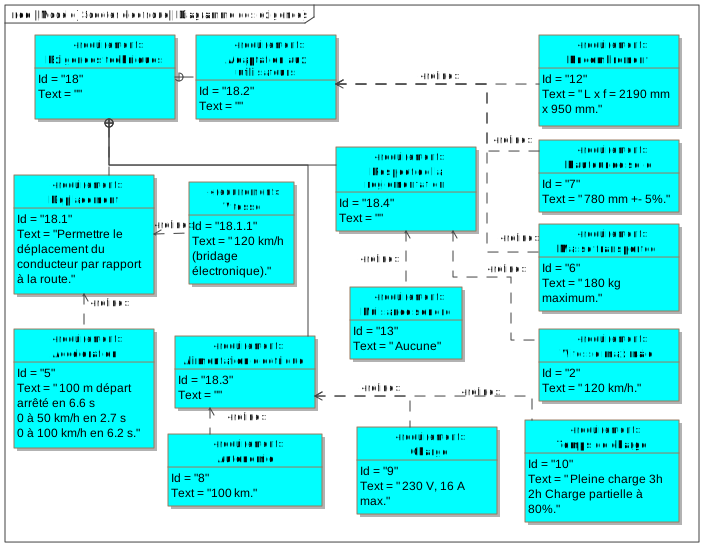
\includegraphics[width=\linewidth]{images/Exigences}
%\end{center}

%La chaîne d’énergie de la Renault Twizy comprend une batterie au Lithium, un onduleur, un moteur électrique et
%un réducteur à engrenages. Ce réducteur est relié aux roues arrière par l’intermédiaire d’un différentiel conique
%qui n’est pas étudié dans ce sujet.

\begin{center}
\includegraphics[width=\linewidth]{images/ccmp_07_bis}
\end{center}


\subsection*{Modélisation de la mise en mouvement du véhicule}
%\subsection{Présentation générale}
\begin{obj}
Utiliser un modèle pour valider le choix de la machine électrique et du réducteur associé.
\end{obj}


Le véhicule est équipé d’une machine électrique asynchrone alimentée par la batterie via un onduleur. Les
commandes actuelles de ces machines permettent de se rapprocher du comportement d’une machine à courant
continu.
On utilise le modèle d’une machine à courant continu en mode moteur. 

%\begin{multicols}{2}
\textbf{Mode moteur :}
\begin{itemize}
\item $u_m(t)=e(t)+R_m i(t)+L_m \dfrac{\dd i(t)}{\dd t}$;
\item $c_m(t)=k_m i(t)$;
\item $e(t)=k_m\omega_m(t)$.
\end{itemize}
\textbf{Mode génératrice :}
\begin{itemize}
\item $e(t)=u_a(t)+R_m i(t)+L_m \dfrac{\dd i(t)}{\dd t}$;
\item $c_m(t)=k_m i(t)$;
\item $e(t)=k_m\omega_m(t)$.
\end{itemize}
%\end{multicols}

Une boucle de courant permet d’éviter une surcharge de la machine électrique.
Nous rappelons l’équation de mouvement nécessaire pour la suite de l’étude : 
$$\dfrac{r}{R}C_m(t)-F_r(t)=M_{\text{eq}}\dfrac{\dd v(t)}{\dd t}.$$

Le modèle du système est donné par le schéma bloc suivant.

\begin{center}
\includegraphics[width=\linewidth]{images/ccmp_01}
\end{center}




On a $C(p)=R_m\left( 1+\dfrac{R_m}{L_m p}\right)$ le correcteur PI de la boucle de courant.

\begin{minipage}[c]{.65\linewidth}
Le comportement du hacheur de fonction de transfert $H(p)$ en fonction de $u(t)$ est :
\begin{itemize}
\item $u_m(t) = u(t)$ si $u (t) \leq U_{\text{max}}$;
\item $u_m(t) = U_{\text{max}}$ si $u (t) > U_{\text{max}}$.
\end{itemize}
\end{minipage} \hfill
\begin{minipage}[c]{.3\linewidth}
\begin{center}
\includegraphics[width=\linewidth]{images/ccmp_02}
\end{center}
\end{minipage}

\subsubsection*{Détermination du temps de réponse du véhicule lors de l’accélération avec une consigne de courant constante}

\begin{obj}
Mettre en place un modèle pour déterminer le temps de réponse du véhicule lors d’une accélération.
\end{obj}

\subsubsection*{Détermination de la réponse en vitesse dans le cas où $u_m(t) \leq U_{\text{max}}$}

\subparagraph{}
\textit{Appliquer la transformée de Laplace à l’équation de mouvement rappelée en début de section, lors d’une accélération. En déduire $A(p)$ et $B(p)$.}
\ifprof
\begin{corrige}
D'après le schéma-blocs, on a $V(p)=B(p)\left(A(p)C_m(p)-F_r(p) \right)$. Par ailleurs, 
on a $\dfrac{r}{R}C_m(p)-F_r(p)=M_{\text{eq}} pV(p)$ $ \Leftrightarrow  \dfrac{1}{M_{\text{eq}} p} \left(\dfrac{r}{R}C_m(p)- F_r(p)\right)=V(p)$. On a donc $B(p)=\dfrac{1}{M_{\text{eq}} p}$ et $A(p)=\dfrac{r}{R}$.
\end{corrige}
\else
\fi


\subparagraph{}
\textit{Calculer, si $F_r(p) = 0$, la fonction de transfert $\dfrac{I(p)}{I_c(p)}$ avec les paramètres du schéma-blocs, puis en remplaçant $A(p)$ et $B(p)$ à l’aide de la question précédente.}
\ifprof
\begin{corrige}
En raisonnant à partir du schéma-blocs, on a $U_m(p)=\left(I_c(p)-I(p)\right)C(p)H(p)$. 

De plus $I(p)=\varepsilon_v(p)\dfrac{1}{R_m + L_m p}=\left(U_m(p)-V(p) K_m A(p) \right)\dfrac{1}{R_m + L_m p}$ et $V(p)=K_m A(p) B(p) I(p)$. 

On a donc : 
$I(p)=\varepsilon_v(p)\dfrac{1}{R_m + L_m p}=\left(\left(\left(I_c(p)-I(p)\right)C(p)H(p) \right)-K_m A(p)^2B(p) I(p) K_m  \right)\dfrac{1}{R_m + L_m p}$


$I(p)=\left(I_c(p)C(p)H(p)-I(p)C(p)H(p) -K_m A(p)^2B(p) I(p) K_m  \right)\dfrac{1}{R_m + L_m p}$


$\Leftrightarrow I(p)\left( R_m + L_m p+C(p)H(p)+K_m A(p)^2B(p) K_m\right)=I_c(p)C(p)H(p) $

$\Leftrightarrow \dfrac{I(p)}{I_c(p)}=\dfrac{C(p)H(p)}{ R_m + L_m p+C(p)H(p)+K_m^2 A(p)^2B(p) }$

$\Leftrightarrow \dfrac{I(p)}{I_c(p)}=\dfrac{ R_m\left( 1+\dfrac{R_m}{L_m p}\right)}{ R_m + L_m p+ R_m\left( 1+\dfrac{R_m}{L_m p}\right) +K_m^2 \left(\dfrac{r}{R}\right)^2 \dfrac{1}{M_{\text{eq}} p}   }$
\end{corrige}
\else
\fi


\subparagraph{}
\textit{Calculer le courant en régime établi $I(\infty)$ si $I_c(p)$ est un échelon d’amplitude $I_0$. Montrer alors que $I(\infty) \simeq I_0$ sachant que $\dfrac{L_mK_m^2\left(r/R\right)^2}{R_m^2 M_{\text{eq}}}=5\times 10^{-4} << 1$.}
\ifprof
\begin{corrige} ~\\

On a $I(\infty) =$ $ \lim_{t\to\infty} i(t)=$ 

$ \lim_{p\to 0 } p \dfrac{I_0}{p} \dfrac{ R_m\left( 1+\dfrac{R_m}{L_m p}\right)}{ R_m + L_m p+ R_m\left( 1+\dfrac{R_m}{L_m p}\right) +K_m^2 \left(\dfrac{r}{R}\right)^2 \dfrac{1}{M_{\text{eq}} p}   }$. 

Ainsi $I(\infty) =I_0 \dfrac{ R_m^2}{   R_m^2 + L_m K_m^2 \dfrac{r^2}{R^2M_{\text{eq}}}    } \simeq I_0$.
\end{corrige}
\else
\fi

La constante de temps électrique étant petite devant la constante de temps mécanique on supposera que la condition précédente est toujours vraie.

Le schéma-blocs simplifié du véhicule si $i(t)=i_c(t)$ et $u_m(t)<U_{\text{max}}$ est le suivant.


\begin{center}
\includegraphics[width=\linewidth]{images/ccmp_03}
\end{center}


\subparagraph{}
\textit{En utilisant le schéma-blocs précédent, calculer $V(p)$ en fonction de $I_c(p)$ et $F_r(p)$ puis en utilisant le
tableau suivant, déterminer l’équation de la vitesse $v(t)$ du véhicule dans le cas où $i_c(t)$ et $F_r(t)$
sont des échelons respectivement d’amplitude $I_0$ et $F_0$.}

\begin{center}
\begin{tabular}{|c|c|c|c|c|}
\hline
$f(t)$, $t>0$ & 1 & $t$ & $t^2$ & $e^{-at}$  \\
\hline
$F(p)$ & $\dfrac{1}{p}$ & $\dfrac{1}{p^2}$ & $\dfrac{2}{p^3}$ & $\dfrac{1}{p+a}$ \\
\hline
\end{tabular}
\end{center}

\ifprof
\begin{corrige}
On a $V(p)= \dfrac{rK_m}{RM_{eq}p}I_c(p) - \dfrac{1}{M_{eq}p} F_r(p)$.
Avec $I_c(p) =\dfrac{I_0}{p}$ et $F_r(p) =\dfrac{F_0}{p}$
$V(p)= \dfrac{rK_mI_0}{RM_{eq}p^2} - \dfrac{F_0}{M_{eq}p^2} $.

On a donc $v(t)= \left( \dfrac{rK_mI_0}{RM_{eq}}t - \dfrac{F_0}{M_{eq}}t\right) h(t) $.

\end{corrige}
\else
\fi

\subsubsection*{Détermination du temps de réponse en vitesse à partir de l’instant où $u_m(t)$ atteint $U_{\text{max}}$}

Dans le schéma-blocs, on note pour une variable $x$, $\Delta x(t)=x(t) - x_0$ avec $x_0=x\left(t_0\right)$ et $t_0$ l’instant où $u_m(t)$
atteint $U_{\text{max}}$. En particulier $\Delta v(t) = v(t) -v_0$ avec $v_0$ la vitesse atteinte à la fin de la phase à accélération constante.

\subparagraph{}
\textit{La tension d’alimentation du moteur ne peut pas dépasser une valeur maximale $U_{\text{max}}$. Le
régulateur la limitera automatiquement à cette valeur. Compléter le schéma bloc simplifié du véhicule du
 document réponse si $u_m(t)=U_{\text{max}}$.}
\ifprof
\begin{corrige}
\begin{center}
\includegraphics[width=.95\linewidth]{images/cor_01}
\end{center}

\end{corrige}
\else
\fi

Le modèle précédent a permis de déterminer $\Delta V (p)=H_1(p)\Delta U(p)+H_2(p)F_r(p)$ avec $H_1(p)\simeq \dfrac{\dfrac{1}{K_m r / R}}{1+\dfrac{R_m M_{\text{eq}}}{\left(K_m r /R\right)^2}p}$ et $H_2(p)\simeq \dfrac{\dfrac{R_m}{\left(K_m r /R\right)^2}}{1+\dfrac{R_m M_{\text{eq}}}{\left(K_m r /R\right)^2}p}$.

\subparagraph{}
\textit{Donner le temps de réponse à 5\, \%.}

\ifprof
\begin{corrige}
On a un système du premier ordre de constante de temps $\tau = \dfrac{R_m M_{\text{eq}}}{\left(K_m r /R\right)^2}$. Le temps de réponse à 5\,\% est de $3\tau$. 
\end{corrige}
\else
\fi


\subsubsection*{Temps nécessaire pour passer d’une vitesse nulle à 95\, \% de la vitesse maximale}

\subparagraph{}
\textit{Donner l’allure de la réponse en vitesse du véhicule pour une consigne en courant constante telle que $u_m(t)$ croit de manière monotone jusqu’à $U_{\text{max}}$. Déduire de ce qui précède le temps $t_{\text{max}}$ pour passer
d’une vitesse nulle à 95\, \% de la vitesse maximale en fonction de $r$, $R$, $M_{\text{eq}}$, 
$K_m$, $R_m$, $I_0$, $v_0$ et $F_0$.}
\ifprof
\begin{corrige}
\end{corrige}
\else
\fi

%\subsubsection*{Validation du choix de la machine électrique et du réducteur associé}
%
%\begin{obj}
%Valider le choix de la machine électrique et du réducteur associé. Vérifier le modèle à partir d’une
%mesure sur le véhicule.
%\end{obj}
%
%\subparagraph{}
%\textit{Un calcul numérique utilisant les résultats précédents a permis d’obtenir la courbe du  document
%réponse. Proposer un rapport de transmission permettant de respecter les exigences souhaitées.
%Conclure par rapport au réducteur choisi et donné dans la figure suivante.}
%\ifprof
%\begin{corrige}
%\end{corrige}
%\else
%\fi
%
%\begin{minipage}[c]{.38\linewidth}
%\begin{center}
%\includegraphics[width=.7\linewidth]{images/ccmp_05}
%\end{center}
%\end{minipage} \hfill
%\begin{minipage}[c]{.48\linewidth}
%\begin{itemize}
%\item $Z_4 = \SI{17}{dents}$
%\item $Z_{5a} = \SI{57}{dents}$
%\item $Z_{5b} = \SI{17}{dents}$
%\item $Z_1 = \SI{68}{dents}$
%\end{itemize}
%\end{minipage} 
%
%\subparagraph{}
%\textit{Une mesure réalisée avec la pédale d’accélérateur à 100\, \% est donnée sur le document réponse.
%On définit deux zones particulières de la réponse en vitesse du véhicule : zone 1 entre 0 et \SI{15}{km/h} et
%zone 2 entre 15 et \SI{45}{km/h}. Pour chaque zone de fonctionnement, proposer par identification, un
%modèle littéral de la vitesse du véhicule. Déterminer les valeurs numériques des constantes intervenant
%dans ces modèles (faire les tracés nécessaires). Justifier le choix de la zone 1 grâce à la courbe de couple.}
%\ifprof
%\begin{corrige}
%\end{corrige}
%\else
%\fi

\subsection*{Récupération d'énergie}
\begin{obj}
Étudier la capacité du véhicule à freiner grâce à la récupération de l’énergie.
\end{obj}

La machine électrique fonctionne dans cette situation en génératrice.
L’accumulateur sera modélisé par un condensateur de capacité $C$.
Le modèle du système est donné par le schéma-blocs suivant.


\begin{center}
\includegraphics[width=\linewidth]{images/ccmp_04}
\end{center}


\subsubsection*{Influence de la capacité $C$ sur les performances en décélération par récupération d’énergie}
\begin{obj}
Étudier l’influence de la capacité sur la décélération du véhicule.
\end{obj}

\subparagraph{}
\textit{Justifier les blocs $\dfrac{1}{R_m+L_m p}$ et $\dfrac{1}{Cp}$.}
\ifprof
\begin{corrige}
Le bloc $\dfrac{1}{R_m+L_m p}$ provient de la loi des mailles en mode génératrice selon laquelle $e(t)=u_a(t)+R_m i(t)+L_m \dfrac{\dd i(t)}{\dd t}$.

L'accumulateur étant un modélisé par un condensateur de capacité $C$, on a la loi de comportement $i(t)=C\dfrac{\dd u_a(t)}{\dd t}$. On a donc $I(p)=CpU_a(p)$ et $\dfrac{U_a(p)}{I(p)}=\dfrac{1}{Cp}$.
\end{corrige}
\else
\fi


\subparagraph{}
\textit{On pose $V(p) = H_3(p) V_1(p) + H_4(p) F_r(p)$. Calculer $H_4(p)$.}
\ifprof
\begin{corrige}
Par lecture directe, on a : $V(p)=-\left( F_r(p)  + F(p)\right)\dfrac{1}{M_{eq}p} + V_1(p)$.

Par ailleurs, $\dfrac{U_a(p)}{E(p)}=\dfrac{\dfrac{1}{\left(R_m + L_m p \right)Cp}}{1+\dfrac{1}{\left(R_m + L_m p \right)Cp}}=\dfrac{1}{\left(R_m + L_m p \right)Cp+1}$.


De plus $F(p)=\dfrac{rK_m}{R}Cp U_a (p)$ et $E(p)=\dfrac{rK_m}{R} V(p)$.


On a donc, $F(p)=\dfrac{rK_m}{R}Cp U_a (p)$
 
$= \dfrac{rK_m}{R}Cp \dfrac{1}{\left(R_m + L_m p \right)Cp+1} E(p)$ 

$= \dfrac{rK_m}{R}Cp \dfrac{1}{\left(R_m + L_m p \right)Cp+1} \dfrac{rK_m}{R} V(p)$.


Au final, 

$V(p)=-\left( F_r(p)  + \dfrac{r^2K_m^2Cp}{R^2\left(\left(R_m + L_m p \right)Cp+1\right)}  V(p)\right)\dfrac{1}{M_{eq}p} + V_1(p)$ 

$\Leftrightarrow V(p)\left(1+ \dfrac{1}{M_{eq}p} \dfrac{r^2K_m^2Cp}{R^2\left(\left(R_m + L_m p \right)Cp+1\right)}\right)=-F_r(p)  \dfrac{1}{M_{eq}p} + V_1(p)$.

On a donc, 
$H_4(p)=-\dfrac{1}{M_{eq}p}\cdot\dfrac{M_{eq}p \left( R^2\left(\left(R_m + L_m p \right)Cp+1\right) \right)}{M_{eq}p \left( R^2\left(\left(R_m + L_m p \right)Cp+1\right) \right)+r^2K_m^2Cp}$ 

$H_4(p)=-\dfrac{R^2\left(\left(R_m + L_m p \right)Cp+1\right) }{M_{eq}p  R^2\left(\left(R_m + L_m p \right)Cp+1\right) +r^2K_m^2Cp}$
$=-\dfrac{\left(R_m + L_m p \right)Cp+1 }{M_{eq}p  \left(\left(R_m + L_m p \right)Cp+1\right) +r^2/R^2 K_m^2Cp}$


Remarque : 

$H_3(p)=\dfrac{M_{eq}p \left( R^2\left(\left(R_m + L_m p \right)Cp+1\right) \right)}{M_{eq}p \left( R^2\left(\left(R_m + L_m p \right)Cp+1\right) \right)+r^2K_m^2Cp}$ 


\end{corrige}
\else
\fi

Pour la suite on donne

$H_3(p)=\dfrac{1}{1+\dfrac{\left(K_m r/R\right)^2}{M_{\text{eq}}p}\dfrac{Cp}{\left(R_m + L_m p\right)Cp+1}}$.






\subparagraph{}
\textit{Déterminer, avec le théorème de la valeur initiale, la décélération $a_0$ à l’instant où le véhicule passe en récupération d’énergie avec $F_r (t) = F_0$ et $v_1(t) = v_0$ des constantes. On prendra $L_m = 0$ pour ce calcul car son effet n’est visible que pour un temps très faible (remarque : $v(t)$ vaut initialement $v_0$, soit $v(t) = v_0 + \int a \dd t$ avec
$a(t)=\dfrac{\dd v(t)}{\dd t}$).}
\ifprof
\begin{corrige}
D'une part, on a $V(p) = H_3(p) \dfrac{v_0}{p} + H_4(p) \dfrac{F_0}{p}$.  D'autre part, 
$H_3(p)=\dfrac{1}{1+\dfrac{\left(K_m r/R\right)^2}{M_{\text{eq}}}\dfrac{C}{R_m Cp+1}}$ et 
$H_4(p)=-\dfrac{R_mCp+1 }{M_{eq}p  \left(R_m  Cp+1\right) +r^2/R^2 K_m^2Cp}$. De plus, $A(p)=pV(p)-v_0$

On a donc, 
$\lim\limits_{t\to 0} a(t)=\lim\limits_{p\to \infty} pA(p)=\lim\limits_{p\to \infty} p\left(pV(p)-v_0\right)$
$=\lim\limits_{p\to \infty} p \left( pH_3(p) \dfrac{v_0}{p} + pH_4(p) \dfrac{F_0}{p}-v_0\right)$

$=\lim\limits_{p\to \infty} p \left( H_3(p) {v_0} + H_4(p) F_0-v_0\right)$
$=\lim\limits_{p\to \infty}   \dfrac{p}{1+\dfrac{\left(K_m r/R\right)^2}{M_{\text{eq}}}\dfrac{C}{R_m Cp+1}}  {v_0} -\dfrac{R_mCp+1 }{M_{eq}  \left(R_m  Cp+1\right) +r^2/R^2 K_m^2C} F_0 -v_0p$

$=\lim\limits_{p\to \infty}   pv_0 \left( \dfrac{R_mCp+1}{R_mCp+1+\dfrac{C\left(K_m r/R\right)^2}{M_{\text{eq}}}} -1  \right) -\dfrac{R_mCp+1 }{M_{eq}  \left(R_m  Cp+1\right) +r^2/R^2 K_m^2C} F_0$

$=\lim\limits_{p\to \infty}  pv_0 \left( \dfrac{-\dfrac{C\left(K_m r/R\right)^2}{M_{\text{eq}}}}{R_mCp+1+\dfrac{C\left(K_m r/R\right)^2}{M_{\text{eq}}}} \right)-\dfrac{ F_0}{M_{eq}} $
$=\lim\limits_{p\to \infty}  pv_0 \left( \dfrac{-\dfrac{C\left(K_m r/R\right)^2}{M_{\text{eq}}}}{R_mCp} \right)-\dfrac{ F_0}{M_{eq}} $


$=   -\dfrac{v_0\left(K_m r/R\right)^2}{M_{\text{eq}}R_m} -\dfrac{ F_0}{M_{eq}} $

\end{corrige}
\else
\fi



\subparagraph{}
\textit{Déterminer la vitesse du véhicule $v_{\infty}$ en régime établi si $F_r (t) = 0$ et $v_1(t) = v_0$ des constantes. Conclure sur l’influence de la capacité $C$ du condensateur sur le freinage avec récupération d’énergie.}
\ifprof
\begin{corrige}

On a donc, 
$\lim\limits_{t\to \infty} v(t)=\lim\limits_{p\to 0} pV(p)=\lim\limits_{p\to 0} pV(p)=\lim\limits_{p\to 0} p H_3(p) \dfrac{v_0}{p}$

$=\lim\limits_{p\to 0}   \dfrac{v_0}{1+\dfrac{\left(K_m r/R\right)^2}{M_{\text{eq}}}\dfrac{C}{R_m Cp+1}} =\dfrac{v_0}{1+\dfrac{\left(K_m r/R\right)^2}{M_{\text{eq}}}C}=\dfrac{v_0M_{\text{eq}}}{M_{\text{eq}}+\left(K_m r/R\right)^2C} $.
\end{corrige}
\else
\fi

\subsubsection*{Validation du modèle et choix technologiques pour le freinage}
\begin{obj}
Vérifier si le freinage par récupération d’énergie est suffisant.
\end{obj}

Le modèle précédent a permis de simuler le comportement du véhicule en récupération d’énergie en fonction de la charge $C$ de l’accumulateur. D’autre part, une mesure de décélération a été réalisée sur le véhicule avec une consigne de vitesse nulle et une vitesse initiale proche de \SI{45}{km/h}.

\subparagraph{}
\textit{Déterminer à partir des courbes issues de la simulation (voir courbes fournies sur le document réponse) les temps nécessaires pour réduire la vitesse de 30\, \% puis 50\, \%. (Faire les tracés nécessaires). Comparer les résultats obtenus par simulation à la mesure fournie sur le document réponse. Conclure sur le modèle utilisé et en particulier sur le résultat de la question précédente.}
\ifprof
\begin{corrige}
\end{corrige}
\else
\fi



\subparagraph{}
\textit{Justifier que le freinage par récupération d’énergie est insuffisant. Quel organe supplémentaire
serait indispensable pour assurer la sécurité.}
\ifprof
\begin{corrige}
\end{corrige}
\else
\fi


\end{multicols}
%
%
%\newpage
%
%\begin{center}
%%\includegraphics[width=\linewidth]{images/cor_01}
%%\textit{}
%\end{center}
%
%
%\begin{center}
%%\includegraphics[width=\linewidth]{images/cor_02}
%%\textit{}
%\end{center}


%
%
%\newpage
%
%
%\begin{center}
%	\includegraphics[width=.9\linewidth]{images/cor_01}
%\end{center}
%
%\begin{center}
%	\includegraphics[width=.9\linewidth]{images/cor_02}
%\end{center}
%
%\begin{center}
%	\includegraphics[width=.9\linewidth]{images/cor_03}
%\end{center}
%
%\begin{center}
%	\includegraphics[width=.9\linewidth]{images/cor_04}
%\end{center}

\end{document}

\subparagraph{}\textit{}


\begin{center}
\includegraphics[width=\linewidth]{images/fig_06}
%\textit{}
\end{center}
\begin{center}
\includegraphics[width=\linewidth]{images/img_04}
%\textit{}
\end{center}

